\documentclass{article}

\usepackage[T1]{fontenc}
\usepackage{textcomp}

\usepackage[english]{babel}
\usepackage[utf8]{inputenc}

\usepackage{lmodern}

\usepackage{hyperref}
\hypersetup{breaklinks}
\hypersetup{pdfborder=0 0 0}

\usepackage[babel=true]{microtype}


\usepackage{amsmath}
\renewcommand{\vec}[1]{\mathbf{#1}}
\newcommand{\mat}[1]{\mathbf{#1}}
\DeclareMathOperator{\Prob}{Prob}
\newcommand{\md}{\mathrm{d}}
\newcommand{\me}{\mathrm{e}}
\newcommand{\mT}{\mathrm{T}}

\usepackage{units}
\usepackage{tikz}
\usetikzlibrary{shapes, arrows, calc}  %new
\usepackage{natbib}
\usepackage{hypernat}
\usepackage{float} % new, figure placement

\allowdisplaybreaks[1]

\title{FMDV notes}
\author{Jan Medlock and Erin Gorsich}


\newcommand{\comment}[1]{\textbf{[#1]}}
\DeclareMathOperator{\diag}{diag}


\begin{document}

\maketitle

\section{Model}

We built four models to represent different mechanisms of FMDV persistence African buffalo.  
Our aim is to understand the the relative importance of each mechanism in allowing FMDV persistence. 
All models are stochastic and individual-based; all track the age and sex of each buffalo along with its immune state.
Models differ by which immune statuses are tracked and which events can occur to each buffalo (Figures 1-4).  

\subsection{Null Model: Calf-to-calf transmission}
Under this hypothesis, buffalo are assumed to be immune due to maternal antibodies ($M$), susceptible to infection ($S$), exposed ($E$), infectious ($I$), or recovered ($R$).  
There are 6 events that can occur to each buffalo: death, birth, waning of maternal antibodies, infection, progression and recovery.
The sequence of events is displayed in Figure 1. The distributions describing each event are detailed in section 3.

%The simulations follow a Gillespie algorithm \citep{gillespie_1977}.
\begin{description}
\item[Death] On the birth of new buffalo calf, the age at death of that calf is sampled from the mortality distribution.

\item[Birth] For each female buffalo, the time until she gives birth to a calf is sampled from its distribution.  
This is done when the female is herself born, to find the time until she gives birth to her first calf, and after a birth, to find the time until she gives birth to her next calf.  
A simple Bernoulli sample determines the sex of each calf.

\item[Maternal Immunity Waning (M. waning)] Each new buffalo calf is assumed to be immune to infection due to maternal antibodies: at birth, the duration of maternal immunity is sampled from its distribution.

\item[Infection] For each susceptible buffalo, the time to infection is sampled from its distribution, which depends on the current number of infected buffalo in the population. 
Upon infection, animals move to the exposed class.

\item[Progression] For each exposed buffalo, the duration until they become infectious is sampled from its distribution.  

\item[Recovery] On infection, the time to recovery is sampled from its distribution.
\end{description}

\begin{figure}[H]
  \centering
  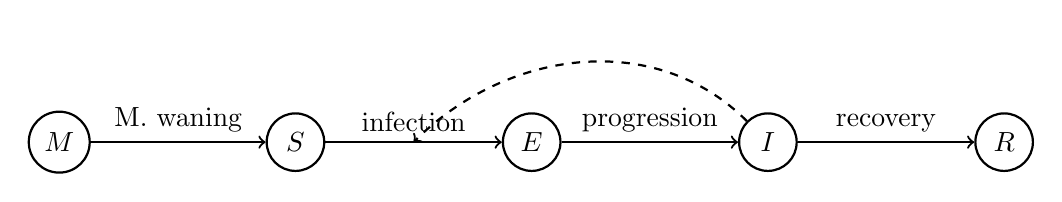
\begin{tikzpicture}[
    thick,
    compartment/.style = {circle,
      draw,
      minimum width = {width("$M$") + 10pt}}
    ]

    \node at (0, 0) [compartment, name = M] {$M$};
    \node at (3, 0) [compartment, name = S] {$S$};
    \node at (6, 0) [compartment, name = E] {$E$};
    \node at (9, 0) [compartment, name = I] {$I$};
    \node at (12, 0) [compartment, name = R] {$R$};

    \draw [->] (M) to node [above] {M. waning} (S);
    \draw [->] (S) to node [above] {infection} (E);
    \draw [->] (E) to node [above] {progression} (I);
    \draw [->] (I) to node [above] {recovery} (R);

    \draw [dashed, ->] (I) to [out = 135, in = 45] ($(S)!0.5!(E)$); %+(0, 0.5) |- +(\x1, 0); 
    
  \end{tikzpicture}
  \caption{Null hypothesis model diagram. Births and deaths are not shown for simplicity. Events are represented with solid lines, influence is represented with dotted lines.  Here, the rate susceptible animals become exposed is influenced by the number of infected animals in the population}
  \label{fig:diagram1}
\end{figure}


\subsection{Alternative Model 1: Waning Immunity (via Evolution)}
Under this hypothesis, recovered buffalo are assumed to lose immunity.  The mechanism is left unspecified as it could be from strain evolution or immunosuppression. The average time buffalo remain recovered is governed by one additional event, waning, and no additional state variables are added. 

\begin{figure}[H]
  \centering
  \tikzstyle{line} = [draw, -latex']
  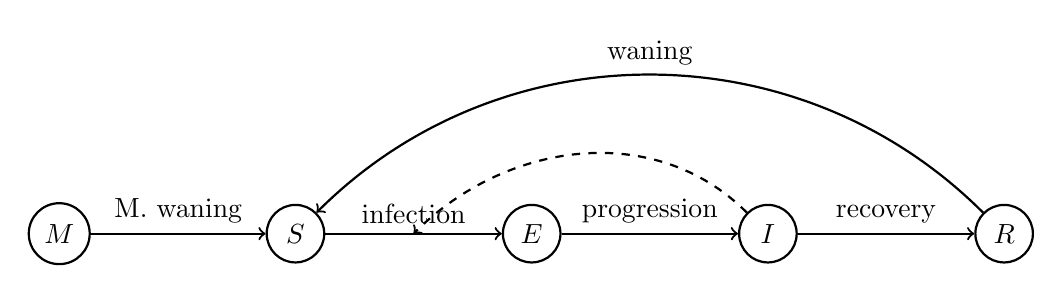
\begin{tikzpicture}[
    thick,
    compartment/.style = {circle,
      draw,
      minimum width = {width("$M$") + 10pt}}
    ]
    \node at (0, 0) [compartment, name = M] {$M$};
    \node at (3, 0) [compartment, name = S] {$S$};
    \node at (6, 0) [compartment, name = E] {$E$};
    \node at (9, 0) [compartment, name = I] {$I$};
    \node at (12, 0) [compartment, name = R] {$R$};

    \draw [->] (M) to node [above] {M. waning} (S);
    \draw [->] (S) to node [above] {infection} (E);
    \draw [->] (E) to node [above] {progression} (I);
    \draw [->] (I) to node [above] {recovery} (R);

    \draw [->] (R) to [out = 135, in = 45]
    node [above] {waning} (S);    
    
    \draw [dashed, ->] (I) to [out = 135, in = 45] ($(S)!0.5!(E)$);
    
  \end{tikzpicture}
  \caption{Alternative Hypothesis 1: Waning immunity model diagram. Births and deaths are not shown for simplicity. Events are represented with solid lines, influence is represented with dotted lines. }
  \label{fig:diagram2}
\end{figure}

\noindent \textbf{Notes from 16-Feb-2017 meeting:} \\
  - The prefered way to model this is to track the strains individually.  This additional detail is Tim's interest so we will leave it for now.   \\
  - The rate of waining should be tied to the number of infections. 
  This can be implemented by specifying the mean waning rate as a function of the current number of infectious individuals, although the functional form needs thought out.  
  Each time an infection occurs, we will have to update the waning event times. 


\subsection{Alternative Model 2: Chronic Carriers}
Under this hypothesis, buffalo remain infectious for the same duration.  
Upon leaving the infected class, a Bernoulli sample with probability, 'probability chronic' determines whether buffalo move to the recoverd class or the chronic carrier class.
The event, chronic recovery, defines the time until buffalo recover from the chronic carrier state.  
Chronic carrier buffalo are assumed to transmit FMDV to influence the force of infection.

\begin{figure}[H]
  \centering
  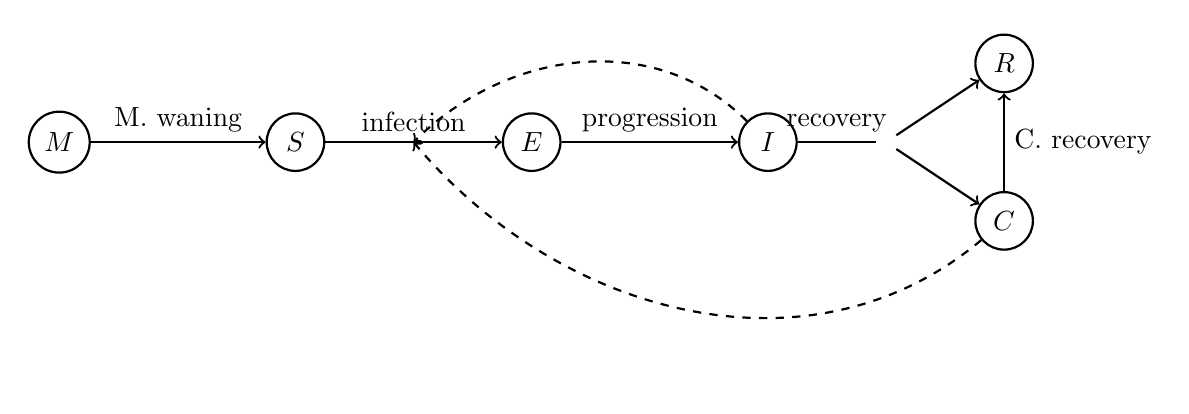
\begin{tikzpicture}[
    thick,
    compartment/.style = {circle,
      draw,
      minimum width = {width("$M$") + 10pt}}
    ]
    \node at (0, 0) [compartment, name = M] {$M$};
    \node at (3, 0) [compartment, name = S] {$S$};
    \node at (6, 0) [compartment, name = E] {$E$};
    \node at (9, 0) [compartment, name = I] {$I$};
    \node at (10.5, 0) [name = dot] {};
    \node at (12, -1) [compartment, name = C] {$C$};
    \node at (12, 1) [compartment, name = R] {$R$};

    \draw [->] (M) to node [above] {M. waning} (S);
    \draw [->] (S) to node [above] {infection} (E);
    \draw [->] (E) to node [above] {progression} (I);
    \draw [->] (dot) to node [above] {} (R);
    \draw [->] (dot) to node [above] {} (C);
    \draw [->] (C) to node [right] {C. recovery} (R);
    \draw [-] (I) to node [above] {recovery} (dot);
    
    \draw [dashed, ->] (I) to [out = 135, in = 45] ($(S)!0.5!(E)$);
    \draw [dashed, ->] (C) to [out = 220, in = 310] ($(S)!0.5!(E)$);

  \end{tikzpicture}
  
  
  \caption{Chronic carriers model diagram. Births and deaths are not shown for simplicity. Events are represented with solid lines, influence is represented with dotted lines. }
  \label{fig:diagram3}
\end{figure}


\noindent \textbf{Notes from 16-Feb-2017 meeting:}  \\
  - Consider representing the fact that transmission from carriers decreases over time.  This can be incorporated with the transmission rate as a function of time since carrier status.  \\
  - This could be estimated from field data as the the proportion of carriers with live virus vs. only RNA in pro bangs.  However, this should be checked for acceptance with the diagnostic team.  
  
\subsection{Alternative Model 3: Waning Immunity and Chronic Carriers}
This hypothesis represents the case where both waning immunity and a carrier state occur.
\begin{figure}[H]
  \centering
  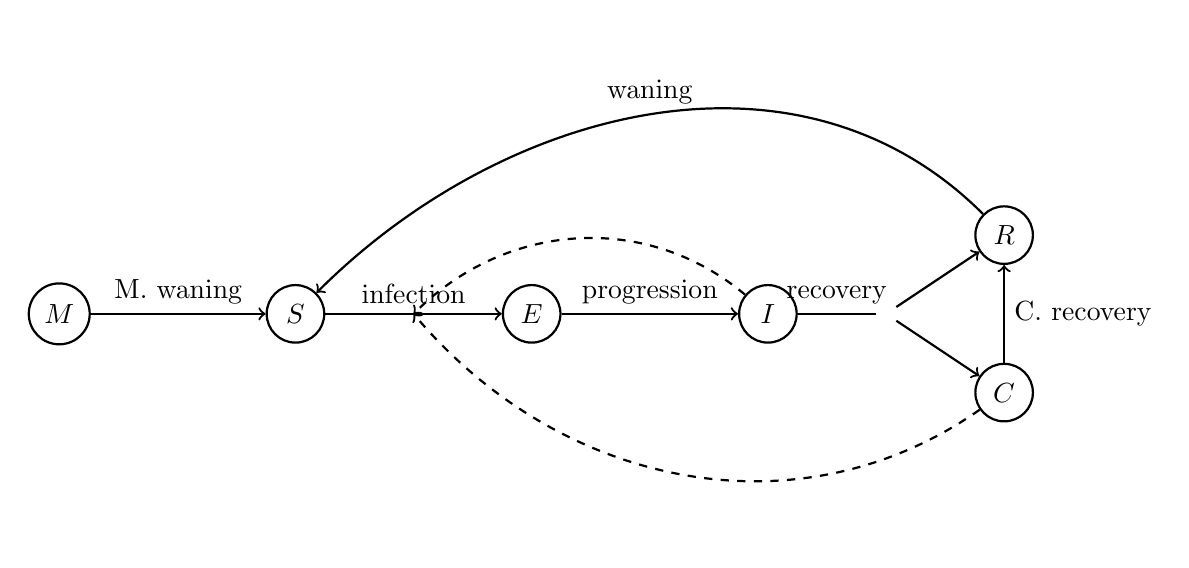
\begin{tikzpicture}[
    thick,
    compartment/.style = {circle,
      draw,
      minimum width = {width("$M$") + 10pt}}
    ]
    \node at (0, 0) [compartment, name = M] {$M$};
    \node at (3, 0) [compartment, name = S] {$S$};
    \node at (6, 0) [compartment, name = E] {$E$};
    \node at (9, 0) [compartment, name = I] {$I$};
    \node at (10.5, 0) [name = dot] {};
    \node at (12, -1) [compartment, name = C] {$C$};
    \node at (12, 1) [compartment, name = R] {$R$};

    \draw [->] (M) to node [above] {M. waning} (S);
    \draw [->] (S) to node [above] {infection} (E);
    \draw [->] (E) to node [above] {progression} (I);
    \draw [->] (R) to [out = 135, in = 45]
    node [above] {waning} (S);    

    \draw [->] (dot) to node [above] {} (R);
    \draw [->] (dot) to node [above] {} (C);
    \draw [->] (C) to node [right] {C. recovery} (R);
    \draw [-] (I) to node [above] {recovery} (dot);
    \draw [dashed, ->] (I) to [out = 140, in = 45] ($(S)!0.5!(E)$);
    \draw [dashed, ->] (C) to [out = 215, in = 310] ($(S)!0.5!(E)$);
  
  \end{tikzpicture}
  \caption{Waning immunity and chronic carriers model diagram. Births and deaths are not shown for simplicity. Events are represented with solid lines, influence is represented with dotted lines. }
  \label{fig:diagram4}
\end{figure}

\section{Parameters}
\begin{table}[ht]
\centering
\begin{tabular}{l c c c c c l c c c}
\hline\hline
Event & Estimate & Distribution & Units & Source\\ [0.5ex]
\hline %\hline
Maternal immunity waning  & $0.5$ & Unif(0.2, 0.8) & yr & ?\\  % needs justified
Infection  & 7.1 & Tr(1.3, 21.1)* & 1/day & Experiment \\
Progression (mean) & 1.2 & Tr(0.1, 4.0) & days & Experiment \\  % Latent period assumed to be gamma distributed.
Progression (shape) & 1 & Tr(0.1, 3.0) & days$^2$ & Experiment\\
Recovery (mean) & 6.0 & Tr(4.0, 8.7) &  days & Experiment \\  % duration of infectious period assumed to be gamma 
Recovery (var) & 3.9 & Tr(1.3, 8.2) & days$^2$& Experiment  \\  % duration of infectious period assumed to be gamma 
Proportion carriers &  0.5 & Unif(0.4, 0.6) &  &  2\\
Infection (from carriers) & 0.78 & Unif(0.01, 3.4) & 1/days & 3\\
Carrier recovery & 0.9 & Unif(0.2, 2.3) & years & 4 \\  
Immunity waning & 5 & Unif(2, 15) & years & ?\\  
\hline
\end{tabular}
\label{table:nonlin}
\end{table}
\noindent 1. ???, 2. Maree et al. 2016  3. Tanzen et al. 2008; 4. Cody and Hedger 1974, Hedger 1972, Anderson et al. 1979, Bengis et al. 1986; 5. ??? \\

\begin{description}
\item[Infection, progression, and recovery]
These estimates and distributions were experimentally estimated from our acute transmission experiment. 
Results from fitting a transmission model to this experimental data showed that individuals were variable in the time they were infectious and the time from exposure to infection.  As a result, progression and recovery are represented with gamma distributions. 
I represent the uncertainty information provided in their estimates with Triangle distributions. Triangle distributions are parameterized with three values, a minimum, maximum, and peak.
QUESTION: Is this OK? - or can we be clever and sample from the posteriors directly with Latin Hypercube?  

\item[Transmission from Carriers]
Our estimate of the transmission rate is based on all chronic carrier experiments for both cattle and buffalo.
Tanzen et al. (2016) estimate the transmission rate from carriers as 0.0256/month.
They report an 85$\%$ CI, so the 95\% bounds presented here are an estimate, and I use uniform to represent this uncertainty.

\item[Duration carrier state]
I summarized data reported in the following studies: Hedger et al. 1972; Condy and Hedger 1974; Anderson et al. 1979; Bengis et al. 1986.
This results in approximate carrier durations for 14 buffalo, although most are censored.  The median and range is reported.
%up to 10 months (292 days; Hedger et al. 1972);  \\
%up to 28 months (Condy and Hedger 1974), with individual infection times of 7, 9, 9, $\>$28, 6, 2 (with last two being flip-flop-ers)
%up to 10m, 24m,  18 months (Anderson et al. 1979)
%up 12-15,  >15, <12, <12 (Bengis et al. 1986)
%Table reports median and published range among individuals.

\item[Maternal Immunity Waning (M. waning)] 
Each new buffalo calf is assumed to be immune to infection due to maternal antibodies. 
At birth, the duration of maternal immunity is set to be 6 months later.  All buffalo lose immunity simultaneously.  \textit{THIS still needs justification}

\item[Proportion Chronic] 
 Maree et al. 2016 summarize as 40- 60\% and Hedger et al. 1972 estimates carriers represent up to 60\% prevalence in the herd.

\item[Waning Immunity] 
Evolution in Vosloo et al. 1996

\end{description}

\section{Expert Questions}
Duration buffalo remain in the 'infected' class (defined by viremia): \\
Duration buffalo remain in the 'infected' class (defined by duration of shedding before a prolonged break): \\
Proportion of buffalo that become carriers (defined as probang positive, viremia negative):
Duration buffalo remain Recovered- e.g. how many days until they can become re-infected:  \\
Duration buffalo remain in the carrier state: \\
Are any of these durations more variable than others?  
If there is lots of individual variation in some processes and not others, we can represent that!


\section{Results}

\section *{Proposed Abstract for ms 2: Alternative mechanisms of persistence}

The persistence of rapidly transmitting pathogens in natural populations represents one of the fundamental puzzles in disease ecology: highly contagious pathogens tend to reduce the pool of susceptible hosts to very low numbers, increasing their own risk of extinction during epidemics troughs. 
Nonetheless, highly transmissible pathogens do occur, despite causing rapid host immunity or mortality.  
In this study, we investigate the epidemiological dynamics of one of the most contagious animal pathogens, foot-and-mouth disease virus (FMDV) in its reservoir host, the African buffalo.  
A key to understanding the epidemiological dynamics is determining the dominant mechanisms of persistence.  
In this work, we present a model representing four alternative hypotheses of how FMDV persists in natural populations: (1) between birth pulses, (2) chronic carriers, (3) viral evolution, and (4) environmental persistence. 
Our results show xxxxx. 
ASK ANNA ABOUT DATA! % say more elegantly. 

%For each buffalo, a list of events and the times they occur is stored.
%The next event over the whole population is found and the population
%s updated.  The hazards for infection depend on the number of
%infectious buffalo in the population and so the times to infection are
%updated after each change in the population.  The hazards of the other
%events are independent of the state of the population and so the times
%to these events are not updated.

%This process was repeated from $t = 0$ to $t = t_{\text{max}}$ or
%until there were $0$ infectious buffalo.

%When sampling from simple distributions, standard algorithms were used
%\citep{scipy}.  For complex distributions, the event times were
%sampled using the inverse transform method \citep{rubinstein_1981}.

%The variables $t$ and $a$ denote time and age, respectively, and are
%both in units of years.

\section{Events and Hazards}


\pagebreak


\bibliography{journal_abbreviations,math_epi}
\bibliographystyle{jpmbib}


\end{document}
